\question{}

\begin{ابجد}
\item طبق تعریف تابع \lr{fitness} در این مسئله داریم:
\begin{align*}
    f(x_1) = 2(5) + (2) + 3(3) - (6) + 2(4) + (1) = 24 \\
    f(x_2) = 2(8) + (1) + 3(7) - (2) + 2(0) + (3) = 39 \\
    f(x_3) = 2(4) + (6) + 3(9) - (1) + 2(2) + (5) = 49 \\
    f(x_4) = 2(9) + (0) + 3(2) - (5) + 2(7) + (8) = 41
\end{align*}
بر اساس مقادیر \lr{fitness} محاسبه شده، مشاهده می‌شود که $x_3$ بهترین عضو در جمعیت اولیه است.

\item عملیات تقاطع (\lr{Crossover}) به این شکل است:
\begin{figure}[htpb]
    \centering
    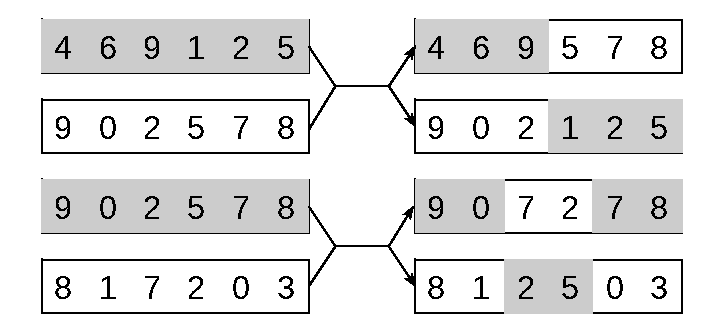
\includegraphics[width=0.5\textwidth]{assets/crossover_diagram.pdf}
    \label{fig:crossover}
\end{figure}

\item عملیات جهش را مطابق با صورت سوال انجام می‌دهیم:
\begin{figure}[htpb]
    \centering
    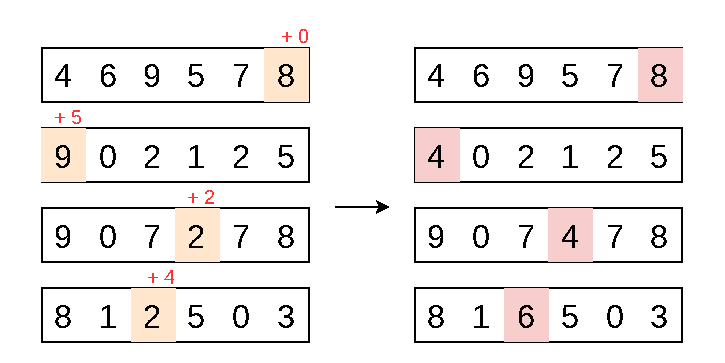
\includegraphics[width=0.5\textwidth]{assets/mutation_diagram.pdf}
    \label{fig:mutation}
\end{figure}

\item ابتدا \lr{fitness} جمعیت جدید را محاسبه می‌کنیم:
\begin{align*}
    f(x_1') = 2(4) + (6) + 3(9) - (5) + 2(7) + (8) = 58 \\
    f(x_2') = 2(4) + (0) + 3(2) - (1) + 2(2) + (5) = 22 \\
    f(x_3') = 2(9) + (0) + 3(7) - (4) + 2(7) + (8) = 57 \\
    f(x_4') = 2(8) + (1) + 3(6) - (5) + 2(0) + (3) = 33
\end{align*}
میانگین جمعیت اولیه و جمعیت جدید را محاسبه می‌کنیم:
\begin{align*}
    \overline{f(x)}  & = \frac{24+39+49+41}{4} = 38.25 \\
    \overline{f(x')} & = \frac{58+22+57+33}{4} = 42.5
\end{align*}
همان طور که انتظار داشتیم، مشاهده می‌شود که میانگین \lr{fitness} در جمعیت جدید بیشتر از جمعیت اولیه است.

\end{ابجد}